\documentclass[draft]{scrartcl}
\title{Simplicial Homology}
\author{Jan Zwank}
\usepackage{amsmath,amssymb,amsthm}
\usepackage[utf8]{inputenc}
\usepackage[T1]{fontenc}
\usepackage{hyperref,microtype,lmodern,csquotes}
\usepackage[english]{babel}
\usepackage{tikz}
\usetikzlibrary{3d,calc,decorations}
\usepackage{pst-solides3d}
\usepackage{caption}

\theoremstyle{plain}
\newtheorem{theorem}{Theorem}[section]
\newtheorem{lemma}[theorem]{Lemma}
\newtheorem{korollar}[theorem]{Korollar}
\newtheorem{satz}[theorem]{Satz}
\newtheorem{hilfssatz}[theorem]{Hilfssatz}
\newtheorem{corollary}[theorem]{Corollary}

\theoremstyle{definition}
\newtheorem	{definition}[theorem]{Definition}
\newtheorem{beispiel}[theorem]{Beispiel}
\newtheorem{beispiele}[theorem]{Beispiele}
\newtheorem{konvention}[theorem]{Konvention}
\newtheorem{notation}[theorem]{Notation}
\newtheorem{axiom}[theorem]{Axiom}
\newtheorem{example}[theorem]{Example}
\newtheorem{examples}[theorem]{Examples}

\theoremstyle{remark}
\newtheorem*{bemerkung}{Bemerkung}
\newtheorem*{bemerkungen}{Bemerkungen}
\newtheorem*{frage}{Frage}

\usetikzlibrary{decorations.markings,intersections}
\tikzset{->-/.style={decoration={
			markings,
			mark=at position #1 with {\arrow[line width=3pt]{stealth}}},postaction={decorate}}}

\newcommand{\SH}{Simplicial Homology}
\newcommand{\sh}{simplicial homology}
\newcommand{\Z}{\mathbb{Z}}
\newcommand{\qandq}{\quad \text{and} \quad}
\newcommand{\qqandqq}{\qquad \text{and} \qquad}
\newcommand{\scs}{simplicial complexes}
\usepackage%[style=authoryear]
	{biblatex}
\bibliography{bibliography}
\begin{document}
	\maketitle
	
	\begin{abstract}
		%TODO 
		Abstract goes here
	\end{abstract}
\tableofcontents

\clearpage

\section{Motivation}\label{motivation}
One of the main goals when studying (topological) spaces (or in this case \scs) is to determine whether two spaces are homotopic
%TODO homeomorphic?
 or not. The first method that is often applied is to check if both spaces are simply connected. A more advanced approach checks not only simply connectedness but also if the fundamental groups $\pi_1$ coincide\footnote{If $X$ is a simply connected space then $\pi_1(X)=0$. Furthermore, the fundamental group is homotopy invariant (up to isomorphism), so homotopic spaces have isomorphic fundamental groups. A more precise formulation of this statement can be found in Hatchers book \parencite[Prop. 1.18, p. 37]{ha}:
\begin{quotation}
	\begin{quote}
		If $\phi: X\to Y$ is a homotopy equivalence, then the induces homomorphism $\phi_*:\pi_1(X,x_0)\to\pi_1(Y,\phi(x_0))$ is an isomorphism for all $x_0\in X$.
	\end{quote}
\end{quotation} }.

It turns out that this is a valuable tool for one and two dimensional \scs. But this method fails for complexes with cells in higher dimensions. It can be shown that the fundamental group actually only depends on the 2-skeleton of the complex \cite[vgl.][p. 173]{ar}. 

Even though this method can be generalized to the study of higher homotopy groups $\pi_n$, this is often more difficult than necessary since the computation of those groups is far from trivial.

In the following we will explore the concept of \sh{} groups and how it can be used to classify spaces. We will see that they allow us to tackle the problem of deciding whether two \textbf{polyhedra}\footnote{A polyhedron is the polytope of a simplicial complex.} are homeomorphic, since simplicial homology is only defined on such spaces. However, the concept of \sh{} can be generalized to singular homology, which can be applied to a broader category of spaces and coincides with \sh{} if both are defined.

However, singular homology groups will not be covered here. The interested reader might refer to the book of Munkres \cite{mu} or Hatcher \cite{ha} to learn more about singular homology groups.

When we concern ourselfes with the question how closed paths on the torus are different from those on the sphere, we can notice the following:

Any Jordan curve (i.e. nonselfintersecting, closed path) on a sphere divides the surface into two \glqq regions\grqq{} as depicted in \autoref{divided-sphere}\footnote{For a more precise statement see \url{https://en.wikipedia.org/wiki/Jordan_curve_theorem}}. The same is not true for the torus. In \autoref{path-on-torus} we see that even tough there are Jordan curves on a torus that bound a \glqq region\grqq of the surface, not all Jordan curves have that property \cite[p. 173f][see]{ar}.

%While we considered all possible paths when we were talking about the fundamental group we will now only consider those that aren't the boundary of a portion of the surface. A great motivation for this approach is given by Armstrong \cite[p. 173f]{ar}:

%Any closed path on the 2-sphere divides the surface into two regions as shown in \autoref{divided-sphere}\footnote{For a more precise statement see \url{https://en.wikipedia.org/wiki/Jordan_curve_theorem}}.

\begin{figure}[h]
	
\parbox{\linewidth}{\parbox[t]{.5\linewidth}{\centering
	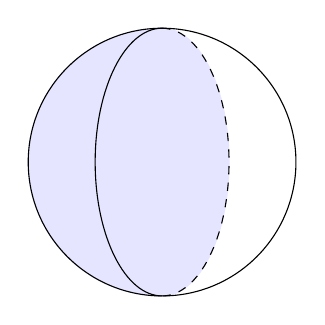
\begin{tikzpicture}[scale=1.7]
		%\draw (-1,0) arc (180:360:1cm and 0.5cm);
		%\draw[dashed] (-1,0) arc (180:0:1cm and 0.5cm);
		\filldraw[blue!10] (0,1)  arc (90:270:1cm) arc (-90:90:0.5cm and 1cm);
		\draw (0,1) arc (90:270:0.5cm and 1cm);
		\draw[dashed] (0,1) arc (90:-90:0.5cm and 1cm);
		\draw (0,0) circle (1cm);
		%\shade[ball color=blue!10!white,opacity=0.20] (0,0) circle (1cm);
	\end{tikzpicture}}%
\parbox[t]{.5\linewidth}{\centering
	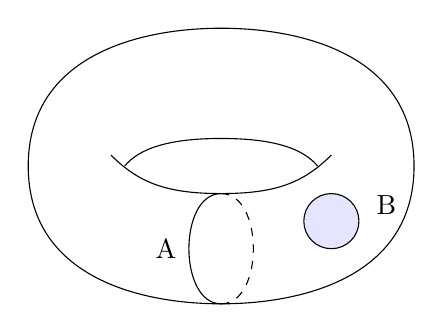
\begin{tikzpicture}[scale=0.7]
	\draw (-3.5,0) .. controls (-3.5,2) and (-1.5,2.5) .. (0,2.5);
	\draw[xscale=-1] (-3.5,0) .. controls (-3.5,2) and (-1.5,2.5) .. (0,2.5);
	\draw[rotate=180] (-3.5,0) .. controls (-3.5,2) and (-1.5,2.5) .. (0,2.5);
	\draw[yscale=-1] (-3.5,0) .. controls (-3.5,2) and (-1.5,2.5) .. (0,2.5);
	
	\draw (-2,.2) .. controls (-1.5,-0.3) and (-1,-0.5) .. (0,-.5) .. controls (1,-0.5) and (1.5,-0.3) .. (2,0.2);
	
	\draw (-1.75,0) .. controls (-1.5,0.3) and (-1,0.5) .. (0,.5) .. controls (1,0.5) and (1.5,0.3) .. (1.75,0);
	
	\draw (0,-0.5) to [out=180, in=180](0,-2.5);
	\draw[dashed] (0,-2.5) to [out=0, in=0](0,-0.5);
	\draw (-1,-1.5) node{A};
	\draw[fill=blue!10!white] (2,-1) circle (0.5);
	\draw (3,-.7) node{B};
	\end{tikzpicture}
%\begin{pspicture}(-6,-4)(6,4)
%\psset{viewpoint=30 0 15 rtp2xyz,Decran=30,lightsrc=viewpoint}
%\psSolid[object=tore,r1=2.5,r0=.7,ngrid=36 72,fillcolor=blue!10!white,grid=false]%
%\end{pspicture}
}}
\parbox[t]{.5\linewidth}{\captionsetup{width=.9\linewidth}
\caption{Any closed path on the sphere divides the surface into two regions.\label{divided-sphere} }}%
\parbox[t]{.5\linewidth}{\captionsetup{width=.9\linewidth}
\caption{There are closed paths on the torus that do not divide the surface into two regions.\label{path-on-torus}}}

\end{figure}

\section{\SH{} Groups with Integer Coefficients}\label{first-hom}

We will use the following definition by Munkres \cite[p. 26]{mu} %and Armstrong \cite[p. 174]{ar}:
\begin{definition}
	For a simplex $\sigma$ we say that two orderings of its vertex set are equivalent if they differ by an even permutation. For a simplex with nonzero dimension, the orderings of the vertices fall into two equivalence classes, called the \textbf{orientations} of $\sigma$. An \textbf{oriented simplex} is a simplex together with an orientation.
\end{definition}
Further we will use the same notation as Munkres \cite[p. 26]{mu}
\begin{notation}
	For geometrically independent points $v_0,\dots,v_p$ we denote the simplex they span with
	\[
	[v_0,\dots,v_p].
	\]
	For an oriented simplex we will use the notation
	\[
	(v_0,\dots,v_p).
	\]
	where the orientation is given by this particular ordering.
%	A change in orientation will be denoted by a minus sign. So, for example
%	\[
%	(v_1,v_2,v_3)=(v_2,v_3,v_1)=(v_3,v_1,v_2)=-(v_1,v_3,v_2)=-(v_2,v_1,v_3)=-(v_3,v_2,v_1)
%	\]
\end{notation}

A choice of orientation is usually depicted with arrows as can be seen in \autoref{orientation-arrows}

\begin{figure}
	\centering

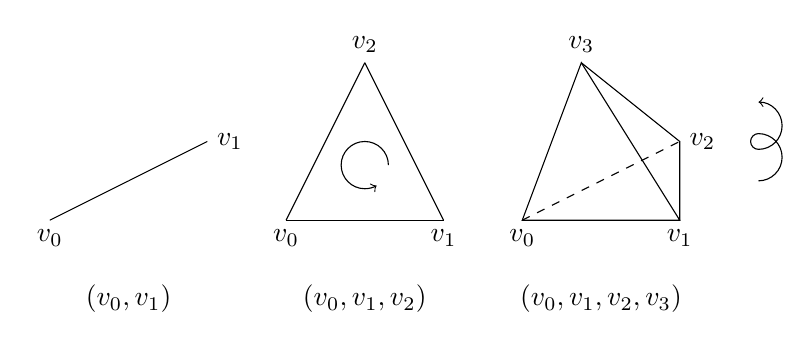
\begin{tikzpicture}
	\draw[] (0,0) node[below]{$v_0$}->(1,0.5);
	\draw (1,0.5)-- (2,1) node[right]{$v_1$};
	\draw (1,-1) node{$(v_0,v_1)$};
	%
	\draw[] (3,0) node[below]{$v_0$}--(5,0)node[below]{$v_1$};
	\draw[] (5,0) -- (4,2) node[above]{$v_2$};
	\draw[] (4,2)--(3,0);
	\draw (4,-1) node{$(v_0,v_1,v_2)$};	
	\draw[->] (4.3,0.7)arc[start angle=0, end angle=300,radius=0.3cm];
	%
	\draw (6,0) node[below]{$v_0$}--(8,0)node[below]{$v_1$}--(6.75,2)node[above]{$v_3$}--cycle;
	\draw (8,0)--(8,1)node[right]{$v_2$}--(6.75,2);
	\draw[dashed] (6,0)--(8,1);
	\draw (7,-1) node{$(v_0,v_1,v_2,v_3)$};
	\draw[->] (9,0.5) arc[start angle=-90, end angle=90, radius=0.3cm] arc [start angle=90, end angle=270,radius=0.1] arc[start angle=-90, end angle=90, radius=0.3];
\end{tikzpicture}
\caption{Indicating orientation with arrows \cite[see][p.27]{mu}\label{orientation-arrows}}
\end{figure}
%
%\begin{definition}
%	The boundary operator of the oriented edge $[v_0,v_1]$ is defined to be the formal linear combination of points
%	\[
%	\partial[v_0,v_1]=v_1-v_0
%	\]
%	and the boundary of the oriented triangle $[v_0,v_1,v_2]$ is defined to be the formal linear combination of edges
%	\[
%	\partial[v_0,v_1,v_2]=[v_1,v_2]-[v_0,v_2]+[v_0,v_1]
%	\]
%\end{definition}
%
%We see that for the closed curve $B$ from \autoref{path-on-torus} with a triangularization as depicted in \autoref{closed-curve} has vanishing boundary, since
%\[
%\partial(a+b+c)=\partial[v_0,v_1]+\partial[v_1,v_2]+\partial[v_2,v_0]=(v_1-v_0)+(v_2-v_1)+(v_0-v_2)=0
%\]
%
%Further, we see that $B$ is indeed the boundary of the interior region, since
%\[
%\partial[v_0,v_1,v_2]=[v_1,v_2]-[v_0,v_2]+[v_0,v_1]=a+b+c
%\]
%
%\begin{figure}\centering
%	\begin{tikzpicture}[scale=2]
%		\draw[fill=blue!10](0,0)--(1,1)--(2,0)--(0,0);
%		\draw node[left]{$v_0$};
%		\draw[->] (0,0)--(0.5,0.5) node[left]{$a$};
%		\draw(0.5,0.5)--(1,1)node[above]{$v_1$};
%		\draw[->](1,1)--(1.5,0.5) node[right]{$b$};
%		\draw (1.5,0.5)--(2,0) node[right]{$v_2$};
%		\draw[->] (2,0)--(1,0) node[below]{$c$};
%		\draw (2,0)--(0,0) node[left]{$v_0$};
%	\end{tikzpicture}
%	\caption{A closed curve triangulated as $[v_0,v_1,v_2]$.\label{closed-curve}}
%\end{figure}
%
%We will now construct the abelian group $Z_1(K)$ by considering all those formal linear combinations of edges with integer coefficients (for now) that satisfy the condition of a vanishing boundary. We  call $Z_1(K)$ the group of 1-cycles.
%
%Similarly, we say that a 1-cycle is a bounding cycle if we can find a linear combination of triangles whose boundary  is the given cycle. The group of such bounding cycles shall be denoted by $B_1(K)$.
%
%Thinking back to the motivational part of this section, we are only \glqq interested \grqq{} in the 1-cycles that aren't also bounding cycles. Obviously, $B_1(K)$ is a subgroup of $Z_1(K)$, so we can form the quotient group
%\[
%H_1(K)=Z_1(K)/B_1(K).
%\]
%This is called the first homology group of $K$.%TODO I never stated what K is.
%
%
%Nowhere in \autoref{first-hom} where we restricted to two dimensions. Actually, the computation of higher simplicial homology groups is very similar to that in 2-dimensions.
%
%We begin with the following definition from Munkres \cite{mu}

To define simplicial homology groups in any meaningful way, we need a few definitions that allow us to formulate our ideas form \autoref{motivation} more precise. There are several ways to go about this with various amounts of rigor. In this paper, we will follow the path of Munkres \cite[p. 27f]{mu}.

%TODO This is a direct citation. Do I need to state that any further?
\begin{definition}
	Let $K$ be a simlicial complex. A \textbf{$p$-chain} on $K$ is a function $c$ from the set of oriented $p$-simplices of $K$ to the integers such that:
	\begin{enumerate}
		\item $c(\sigma)=-c(\sigma^\prime)$ if $\sigma$ and $\sigma^\prime$ are opposite orientations of the same simplex.
		\item $c(\sigma)=0$ for all but finately many oriented $p$-simplices $\sigma$.
	\end{enumerate}
We add $p$-chains by adding their values; the resulting group is denoted $C_p(K)$ and is called the group of (oriented) $p$-chains of $K$. If $p<0$ or $p>\dim K$, we let $C_p(K)$ denote the trivial group.

If $\sigma$ is an oriented simplex, the elementary chain $c$ corresponding to $\sigma$ is the function defined as follows:
\begin{align*}c(\sigma)=&1,\\
 c(\sigma^\prime)=&-1&&\text{ if $\sigma^\prime$ is the opposite orientation of $\sigma$}\\
 c(\tau)=&0 &&\text{ for all other oriented simplices $\tau$.} 
 \end{align*}
\end{definition}

It is common practice to to abuse the notation here. If clear by context we use the symbol $\sigma$ not only to denote the (oriented) simplex, but also the corresponding elementary chain.

We are now able to formulate the our first result as can be found in Munkres book \cite[Lemma 5.1, p. 28]{mu}:
\begin{lemma}
	$C_p(K)$ is free abelian; a basis for $C_p(K)$ can be obtained by orienting each $p$-simplex and using the corresponding elementary chains as a basis.
\end{lemma}
%TODO proof the Lemma
\section{\SH{} Groups with $\mathbb{Z}/2\mathbb{Z}$ Coefficients}
\section{Functoriality Property}
\section{Homotopy Invariance of \SH}

\printbibliography
\end{document}